% sage_latex_guidelines.tex V1.20, 14 January 2017

\documentclass[Afour,times,sageh]{sagej}

\usepackage{moreverb,url}

\usepackage[colorlinks,bookmarksopen,bookmarksnumbered,citecolor=red,urlcolor=red]{hyperref}

\newcommand\BibTeX{{\rmfamily B\kern-.05em \textsc{i\kern-.025em b}\kern-.08em
T\kern-.1667em\lower.7ex\hbox{E}\kern-.125emX}}

\def\volumeyear{2016}

\begin{document}

\runninghead{Zhang et al.}

\title{SAMPLE PAPER}

\author{Jesse Zhang\affilnum{1}, Jiangyi Xia\affilnum{1}, John Olichney \affilnum{1}}

\affiliation{\affilnum{1}UC Davis Center for Mind and Brain}

\corrauth{}

\email{jessezhang@berkeley.edu}

\begin{abstract}
We present an approach for electroencephalogram (EEG)-based classification between mild cognitively impaired patients that later converted to Alzheimer's (MCI-C) and robust normal elderly (RNE) via a graph theory approach with visibility graphs (VG). This approach is based on previous research that has demonstrated  differences between patients with MCI or Alzheimer's and normal elderly people in terms of word repetition trial EEG peak amplitudes. The EEG signals are wavelet decomposed into 5 sub-bands ($\alpha, \beta, \delta, \gamma, \theta$) and 1 raw signal, then converted to VGs for analysis. Twelve graph features are tested for group differences between the MCI-C and RNE groups, and t-testing is employed for feature selection. The features are then classified with a deep neural network (DNN) after mathematical dimensionality reduction, resulting an a high classification accuracy of 99.75\% over 100 iterations of training and testing. The same DNN model was then used to classify an independent set of Alzheimer's patients with an accuracy of 99.17\%.
\end{abstract}

\keywords{}

\maketitle
\section{Introduction}
\textbf{Placeholder for now}
Mild Cognitive Impairment (MCI) is an important research entity as it is often regarded as "prodromal Alzheimer's," the leading cause of dementia in our elderly population. On average, patients with MCI convert to Alzheimer's (AD) at a rate of 12.5\% per year, affording researchers the challenge (and opportunity) of finding new measures that improve our ability to reliably diagnose AD earlier......

Electroencephalogram (EEG) has been shown (cite Olichney papers) to ...measures of early detection.....

We utilized a type of computational graph called a Visibility Graph (VG), which preserves many features of the original EEG signal, in the analysis presented here. Converting resting state EEG signals to VGs allows for discriminative graph features to be utilized in high-accuracy neural network based classification (98\%) between AD patients and robust normal elderly (RNE) \citep{Ahmadlou2010}. Our hypothesis is that word repetition tasks, which are known to reveal significant differences between MCI-C and RNE groups (\citet{OlichneyN400}, \citet{OlchneyP600}, \citet{TaylorERP}), can also demonstrate differences when the corresponding EEG signals are converted to VGs. We then applied a similar approach, testing many more features, to word repetition task EEG signals to classify between patients with MCI that converted to Alzheimer's at a later date (MCI-C) and RNE. We finally verified these results by testing if the same features could discriminate between word repetition task EEG signals of Alzheimer's patients and our RNE and utilized said features to classify between AD patients and RNE.
\begin{abstract}
<Text>
\end{abstract}

\keywords{<List keywords>}

\maketitle
% \section{The article header information}
% The heading for any file using \textsf{\journalclass} is shown in
% Figure~\ref{F1}. You must select options for the trim/text area and
% the reference style of the journal you are submitting to.
% The choice of \verb+options+ are listed in Table~\ref{T1}.

% \begin{table}[h]
% \small\sf\centering
% \caption{The choice of options.\label{T1}}
% \begin{tabular}{lll}
% \toprule
% Option&Trim and font size&Columns\\
% \midrule
% \texttt{shortAfour}& 210 $\times$ 280 mm, 10pt& Double column\\
% \texttt{Afour} &210 $\times$ 297 mm, 10pt& Double column\\
% \texttt{MCfour} &189 $\times$ 246 mm, 10pt& Double column\\
% \texttt{PCfour} &170 $\times$ 242 mm, 10pt& Double column\\
% \texttt{Royal} &156 $\times$ 234 mm, 10pt& Single column\\
% \texttt{Crown} &7.25 $\times$ 9.5 in, 10pt&Single column\\
% \texttt{Review} & 156 $\times$ 234 mm, 12pt & Single column\\
% \bottomrule
% \end{tabular}\\[10pt]
% \begin{tabular}{ll}
% \toprule
% Option&Reference style\\
% \midrule
% \texttt{sageh}&SAGE Harvard style (author-year)\\
% \texttt{sagev}&SAGE Vancouver style (superscript numbers)\\
% \texttt{sageapa}&APA style (author-year)\\
% \bottomrule
% \end{tabular}
% \end{table}

% For example, if your journal is short A4 sized, uses Times fonts and has Harvard style references then you would need\\
% {\small\verb+\documentclass[ShortAfour,times,sageh]{sagej}+}

% Most \textit{SAGE} journals are published using Times fonts but if for any reason you have a problem using Times you can
% easily resort to Computer Modern fonts by removing the
% \verb"times" option.

% \subsection{`Review' option}
% Some journals (for example, \emph{Journal of the Society for Clinical Trials}) require that
% papers are set single column and with a larger font size to help with the review process.
% If this is a requirement for the journal that you are submitting to, just add the \verb+Review+ option to the \verb+\documenclass[]{sagej}+ line.

% \subsection{Remarks}
% \begin{enumerate}
% \item[(i)] In \verb"\runninghead" use `\textit{et~al.}' if there
% are three or more authors.

% \item[(ii)] For multiple author papers please note the use of \verb"\affilnum" to
% link names and affiliations. The corresponding author details need to be included using the
% \verb+\corrauth+ and \verb+\email+ commands.

% \item[(iii)] For submitting a double-spaced manuscript, add
% \verb"doublespace" as an option to the documentclass line.

% \item[(iv)] The abstract should be capable of standing by itself,
% in the absence of the body of the article and of the bibliography.
% Therefore, it must not contain any reference citations.

% \item[(v)] Keywords are separated by commas.

% \item[(vi)] If you are submitting to a \textit{SAGE} journal that requires numbered sections (for example, IJRR), please add the command
%   \verb+\setcounter{secnumdepth}{3}+ just above the \verb+\begin{document}+ line.

% \end{enumerate}


 \section{Methods}

 \begin{figure}
 \centering

\includegraphics[width=0.36\textwidth]{figures/MCI_Olichney_Methods}
\caption{Flowchart of entire analytic process}
\label{Methods}
 \end{figure}
 
 Figure \ref{Methods} details the entire research methodology from start to finish.
 Code for the methods described below is available online at \href{https://github.com/jesbu1/MCI-Visibility-Graph-ML}{https://github.com/jesbu1/MCI-Visibility-Graph-ML}.
 \subsection{Participants}
 EEG and behavioral data were taken from 25 patients with amnestic MCI (10 MCI non-converters: mean age 71.1 year, range 55-81; 15 MCI converters: mean age 74.6 year, range 60-84) and 11 healthy elderly controls (mean age 74.1 years, range 57-79) who were recruited in a previous published longitudinal study \citep{OlchneyP600}. The patients were recruited primarily through the Shiely-Marcos Alzheimer’s Disease Research Center (ADRC) at the University of California, San Diego. All participants were screened for treatable causes of cognitive impairments such as vitamin B12 deficiency and thyroid dysfunction, and underwent a brain scan (generally MRI) prior to enrollment. The exclusion criteria included stroke, epilepsy, psychiatric conditions, as well as several classes of CNS-active medications. 
The patients were tested annually with a EEG word repetition paradigm and clinical assessments. At the initial baseline recording session, the patients all met the Petersen Criterion for MCI \citep{PetersonMCI}, but not for dementia \citep{APA}. Out of the 25 MCI patients, 15 subsequently converted to AD within 3 years of their initial baseline session (mean number of years $1.62 \pm 0.7$). Conversion to AD was defined according to the criteria set out by the National Institute of Neurological and Communicative Disorders and Stroke-Alzheimer’s Disease and Related Disorders Association \citep{McKhann}. In the present study we focus on the initial baseline EEG and neuropsychological assessment data in order to investigate neural activity predictive of MCI to AD conversion in the following 3 years. For more information about participant demographics and neurocognitive testing please refer to \citet{OlichneyN400}.
\subsection{Word Repetition Paradigm}
For each trial, participants were presented with an auditory phrase describing a category (e.g., ``a type of wood", ``a breakfast food") followed by a visually presented target word $\sim$1 s later (presentation duration = 0.3 s, visual angle $\sim =$ 0.4$^{\circ}$). The target words were either congruous or incongruous with the preceding category phrase with a probability of 0.5. Congruous and incongruous words were matched on the frequency of usage (mean = 32, SD = 48; \citet{kucera}) and word length (mean of 5.8 characters, SD = 1.6). Participants were instructed to wait for 3 s after the onset of each target word, read the word aloud, and then give a yes/no decision indicating whether the word fit the preceding category. No time limit was imposed on making responses. Of all the category-word pairs, 1/3 only appeared once, 1/3 appeared twice, and the other 1/3 appeared 3 times (congruous and incongruous pairs were counterbalanced). For those items appeared twice, the lag between the first and the second presentation was short (0-3 intervening trials, spanning $\sim$10-40 s). For those items appeared 3 times, the lags between presentations were longer (10-13 intervening trials, spanning $\sim$100-140 s). A total of 432 trials were performed in 3 blocks. Further details of the experimental paradigm have been published previously (\citet{Olichney2000}, \citet{OlchneyP600}). 
\subsection{Wavelet Decomposition and EEG Signal Preparation}
Across participants, EEG was recorded from 19 to 32 channels including midline (Fz, Cz, Pz) and lateral (F7/F8, T5/T6, O1/O2) sites in the International 10-20 System and additional sites approximate Broca area (BL/BR), Wernicke area (WL/WR), and Brodmann area 41 (41L/41R). EEG signals were recorded with a 250 Hz sampling rate, band passed between 0.016 to 100 Hz, and re-referenced offline to averaged mastoids. Data preprocessing and artifact rejection were performed using MATLAB \citep{MatLab} with EEGLAB \citep{EEGLAB} and Fieldtrip \citep{FieldTrip} toolboxes.
EEG epochs were extracted and time-locked to the onset of target words, 2 s before and 2 s after the word onset, and visually inspected for non-physiological artifacts. Independent component analysis \citep{ICA} was then applied to isolate and remove eye movement artifacts. Artifact-removed EEG epochs were then mirror-padded to 8 s (2 s to the beginning and 2 s to the end) and band-pass filtered into seven frequency bands ($\delta$ 1–4 Hz, $\theta$ 4–8 Hz, $\alpha$ 8–13 Hz, $\beta$ 13–30 Hz, $\gamma$ 30–45 Hz), using zero-phase Hamming-windowed since FIR filters as implemented in the EEGLAB ($pop_eegfiltnew$). This function automatically selects the optimal filter order and transition band width to minimize filter distortions and maximize time precision. Finally, raw and band-pass filtered EEG segments were extracted 1 s before and 2 s after the word onset for further analyses.

\subsection{Time series to visibility graph conversion:}
For every patient, all trials under each condition, channel, and band combination were averaged to produce a single, averaged time series in order to reduce the effects of noise and vastly improve the amount of time required to run analysis. Each time series was then averaged into 80 ms non-overlapping epochs (the values of every 20 timesteps were averaged together). This was done in order to keep amount of memory and processing power required to extract features feasible enough for our computer (MacBook Pro 2.7 GHz Dual Core i5 with 8GB RAM) to run in a reasonable amount of time. All time series were finally shortened to 1 second pre-stimulus to 2 seconds post-stimulus.
\subsection{Visibility Graphs (VG)}
Visibility Graphs (VG), first proposed by \citet{Lacasa2008}, inherit many properties of the time series they represent. For example, a visibility graph corresponding to a periodic series will be a regular graph and a random series will be a random graph. Visibility Graphs were first utilized in EEG analysis in a paper by Ahmadlou et al. \citep{Ahmadlou2010} in order to classify Alzheimer’s patients against controls, with a classification accuracy of 97.8\%.

Intuitively, a visibility graph of a time series \textbf{x} is created by considering each $i$'th point of the time series and determining which other time points are visible from it. The $i$'th node of the VG will be connected with an undirected  edge to any nodes visible from it. Formally, two nodes of the VG, $a_m$ and $a_n$, are connected with an undirected, weight 1 edge if and only if: $$x_{m+j} < x_n + (\frac{n-(m+j)}{n-m})(x_m - x_n)$$ $$ \forall j \in \mathbb Z_+ : j < n - m$$
Figure \ref{VG} demonstrates the creation of a VG. The top graph represents the original time series, while the graph underneath represents the corresponding nodes and edges of the visibility graph. There is a line connecting points in the time series (and an undirected edge in the corresponding VG) if and only if those two points are visible from each other.
\begin{figure}
 \centering
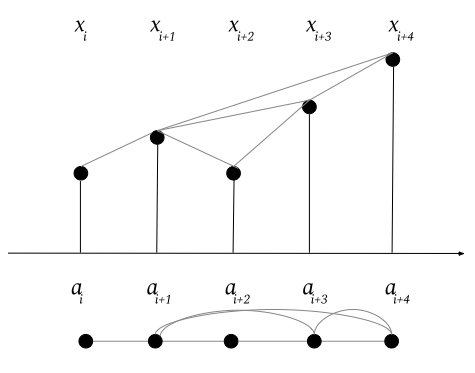
\includegraphics[width=0.5\textwidth]{figures/VG}
\caption{The top graph represents a time series, and the edges between points signify which points can see each other. The bottom graph represents the VG of the time series, with nodes corresponding to timepoints and edges corresponding to lines of visibility}
\label{VG}
 \end{figure}
\subsection{Feature Extraction}
In total, 12 features were selected to be analyzed for significant differences across the MCI Converter (MCI-C) and the robust normal elderly (RNE) groups. 6 of these features, namely clustering coefficient sequence similarity, average clustering coefficient, global efficiency, local efficiency, small-worldness, and graph index complexity have been tested in previous Alzheimer’s EEG graph theory studies (\citet{Ahmadlou2010}, \citet{Wang2016}, \citet{Wang2017}, \citet{Kabbara}, \citet{Haan2009}). The other 6 are graph features heavily studied in the field of computer science that,  as far as the authors are aware of, have not yet been analyzed in EEG graph theory studies. Every feature was extracted from each condition, band, and channel combination and then compared across groups with a two-tailed t-test. The entire feature extraction process was performed in Python 3 using Numpy, Scipy, and NetworkX, three open source packages that were essential for data formatting, t-testing, and graph analysis. In all definitions below, $|V|$ denotes the number of vertices in the graph, and $|E|$ denotes the number of edges.
\subsection{Clustering Coefficient Sequence Similarity (CCSS)}
All visibility graphs are constructed from a single time series (an single-channel EEG signal), making it easy to compare individual time series across groups. Visibility graph similarity, proposed by Ahmadlou et al. \citep{Ahmadlou2012} and modified for EEG VG analysis by Wang et al. \citep{Wang2016}, is a method of comparing the similarity of multiple time series across groups by measuring the similarity of the degree sequences in the VGs. As suggested by Wang et al., the similarity of clustering coefficient is utilized instead of degree sequences to generate connections between the visibility graphs of different channels under a single band-condition combination \citep{Wang2016}. Networks are generated by making each channel a node, and connecting an edge between two nodes if the CCSS between their VGs is above a certain threashold, $\theta$, which was chosen to be 0.25 based on Wang's results and our own empirical data. CCSS between two VGs $X$ and $Y$ is calculated as follows: $$CCSS = |\frac{cov(CCS(X), CCS(Y))}{\sigma_{CCS(X)} \sigma_{CCS(Y)}}|$$ The average number of edges between our two groups was compared in t-testing.
\subsection{Average Clustering Coefficient}
The local clustering coefficient of a vertex measures how close the vertex's neighbors are to becoming a complete graph (clique) \citep{Watts}. The clustering coefficient $C$ of a node $i$ is defined as:  $$C_i = \frac{2|E_i|}{|K_i|(|K_i| - 1)}$$where $|E_i|$ denotes the number of edges of the neighbors of a node $i$, $|K_i|$ indicates the number of neighbors of node $i$, and $\frac{|K_i|(|K_i| - 1)}{2}$ represents the number of possible connections in a complete graph consisting of node $i$'s neighbors. Thus, the average clustering coefficient is defined as $$C = \frac{1}{|V|} \sum_{i=1}^{|V|} C_i$$ The average clustering coefficient measures the average tendency of neighbors of nodes to become complete graphs. In context, it denotes the likelihood of our EEG signals to be shaped in a way that allows for close interconnectedness in the VG.
\subsection{Global Efficiency}
Global efficiency is defined as the average of the inverse shortest path lengths between all nodes. The shortest path length $d_{ij}$ between two nodes in our VG construction, $i$ and $j$, is defined to be the minimum number of edges needed to traverse from $i$ to $j$ or $j$ to $i$. Thus global efficiency $E_{global}$, is the defined as  $$E_{global} = \frac{1}{|V|(|V| - 1)} \sum_{i, j, i \neq j} \frac{1}{d_{ij}}$$ It's interpreted as sum of all inverse shortest paths distances divided by the number of shortest paths distances counted [9]. A higher global efficiency corresponds to a network that is more efficient at transmitting/combining information and relates to the small-worldness of the network (\citet{Wang2016}, \citet{Kabbara}, \citet{Latora}, \citet{Rubinov2010}, \citet{Stam2007}, \citet{Harrington2015}). In context, a higher global efficiency in a VG means that there are likely more EEG time points that are visible from other points which are relatively farther away in time.
\subsection{Local Efficiency}
The local efficiency of a graph is the average of the global efficiencies of each subgraph composed of every vertex’s direct neighbors. It’s similar to the average clustering coefficient, however during its calculation, vertices outside of each subgraph can be taken into account in the shortest path between two nodes \citep{Wang2016}. Local efficiency, $E_{local}$, is defined as $$E_{local} = \frac{1}{|V|} \sum_{i} \frac{1}{|V_{g_i}|(|V_{g_i}| - 1)} \sum_{j, k, j \neq k} \frac{1}{d_{jk}} $$, where is $|V_{g_i}|$ represents the number of vertices in the subgraph of vertex $i$ (composed only of its direct neighbors) and $|V|$ represents the number of vertices of the entire graph \citep{Latora}. As each edge in our VG is of weight one, a higher local efficiency corresponds to more direct edges on average in each subgraph, indicating EEG signals with variations in voltage that allow for a greater number of direct connections between points close in time.
\subsection{Small-Worldness}
Small-worldness is a measure of how much a graph acts like a small-world network. Small-world networks have the property that the typical distance between any two randomly chosen vertices grows logarithmically in terms of total number of vertices of a graph \citep{Latora}. As logarithmic functions grow very slowly, this corresponds to low average shortest path lengths, and subsequently high global efficiencies and clustering coefficients. A measure of small-worldness, $S$ was defined by Humphries and Gurney \citep{Humphries2008} as $$S = \frac{C/C_r}{L/L_r}$$where $C, C_r$ are the average clustering coefficients of the graph in question and a random graph respectively, and $L, L_r$ are the average shortest paths lengths between all pairs of vertices in the graph in question and the random graph, respectively. Our random graphs were generated with the Erd\"{o}s-R\'{e}nyi method \citep{erdos59a}, and the same random graph was used to compare all VGs.
\subsection{Graph Index Complexity (GIC)}
GIC, proposed by Kim and Wilhelm \citep{Kim2008}, is a measure of graph complexity. It’s defined as $$GIC = 4c(1-c)$$ where $$c = \frac{\lambda_{max} - 2 \cos(\pi / (|V| + 1))}{|V| - 1 - 2 \cos(\pi/(|V| + 1))}$$$\lambda_{max}$ represents the largest eigenvalue of the adjacency matrix of the graph. A larger GIC corresponds to a more complex VG structure, which is related to the structure of the EEG signal.
\subsection{Size of Max Clique}
A clique is a subset of vertices of a graph such that they form a  complete subgraph---all vertices have direct edges to each other \cite{Luce1949}. Therefore a maximum clique is just the clique with the largest number of vertices in the graph. As clique-finding in graph theory is known to be in a class of problems that may always take exponential time to solve \citep{Boppana1992}, a fast approximation algorithm that, in the worst case, overestimates by a factor proportional to $|V|/(\log|V|)^2$ was used \citep{PAPADIMITRIOU1977}. Max clique was selected by the authors as a feature because it can possibly account for a specific cluster of time points in the EEG signal that are shaped differently across groups, leading to a complete subgraph in the VG of differing numbers of vertices.
\subsection{Cost of Traveling Salesman Problem (TSP)}
The traveling salesman problem is asks the question: what is the shortest cost tour in a graph that starts from a vertex, visits all other vertices in the graph, and then returns to the starting vertex \citep{Algorithms}? This problem is also difficult for computers to solve efficiently, therefore an approximation algorithm that overestimates by at most a factor of 2 was implemented \citep{Algorithms}. As all edge weights in our VGs are 1, this essentially amounts to the shortest length tour that visits all vertices, starting and ending at the vertex that corresponds to the first time point of the EEG. The TSP path cost provides another measure of graph complexity that can signify differences in EEG wave structure across groups.
\subsection{Density}
Graph density is a measure of how close a graph is to having the maximum number of edges. It is simply the actual number of edges divided by the maximum possible number of edges \citep{Wijk2010}. Density, $D$, for an undirected graph is defined as $$D = \frac{2|E|}{|V|(|V|-1)}$$as it can have at most $\frac{|V|(|V|-1)}{2}$ edges. Density can highlight differences in the number of edges of VGs across groups, relating to a difference in EEG signal shape.
\subsection{Independence Number}
The independence number is the size of the largest independent set of a graph, which is the largest set of vertices such that no two vertices share an edge \citep{Bollobas}. This can be reduced to the max clique problem \citep{Boppana1992}, therefore a similar approximation algorithm was used to determine the independence number. A higher independence number could indicate an EEG signal shape that allows for more, or different, timepoints to be invisible from each other.
\subsection{Size of Minimum Cut}
In this context, the minimum cut is defined to be a partition of the vertices into two disjoint sets such that the number of edges across the cut is minimized. This feature was analyzed because a difference in minimum cut size across the two groups could indicate timepoints in the EEG signal that are on average more or less visible (therefore having differing numbers of edges) from other vertices.
\subsection{Size of Vertex Coloring}
Vertex coloring describes the problem of finding the minimum number of colors required to color a graph such that no two vertices that share an edge have the same color. We used an approximation algorithm that colors vertices in order from largest to smallest degree as the problem is also extremely difficult to exactly solve \citep{Kosowski}. The number of colors required to color a graph is likely to be different between two graphs if there is a significant difference in graph structure, or in this case, EEG signal structure.
\section{Statistical Analysis and Feature Selection}
As stated in \textit{Feature Extraction}, we utilized a two-tailed t-test, as implemented in the open-source library Scipy, to determine statistical significance in graph features between groups. A $p$-value of 0.01 was determined as the threshold for significance.
\subsection{Feature Selection}
All features with a $p$-value of less than 0.01 were selected, however a high number of feature combinations combined with the fear of a false discovery rate of 1\% lead us to use principal component analysis (PCA), a method of mapping features from a higher dimensional space into a lower one. As suggested by \citet{Ahmadlou2010}, PCA was applied to reduce the dimensionality of the feature space to about 10\% of its original dimensionality. At a high level, PCA reduces the input vector's dimension such that the resulting vector preserves as much of the variation of the original data as possible; it can also be interpreted as a way to project the vector onto a smaller dimension space such that the distance between the original and new features is minimized.

In our research, the input to PCA consists of a vector containing the values for all significant features as discovered by t-testing. The input is first standardized, and the final output dimension was selected from testing different values around 10\% of the number of original features.
\section{Classification}
We created a deep neural network (DNN) (\citet{Islam2017}, \citet{Zhao2014}, \citet{Morabito2016}) in which the inputs were vectors produced by PCA and the output is 0 or 1, for RNE or MCI-C respectively. We utilized two hidden layers, the first having the same size as the number of features of the input, the second having double the number of nodes as the previous. The number of nodes of the input layer is the same as the dimension of the vector produced by PCA. Figure \ref{NN} demonstrates an example DNN  of this structure. A ReLU activation function, which just outputs the max of the input value and 0 (\citet{Xu2015}, \citet{Hahnloser2000}), was applied to the inputs to both hidden layers and a sigmoid function to the input of the output neuron in order to produce a value between 0 and 1. The weights of the neural network are obtained by training it to minimize classification error as calculated by the cross entropy loss function \citep{deBoer2005}. 
\begin{figure}
 \centering
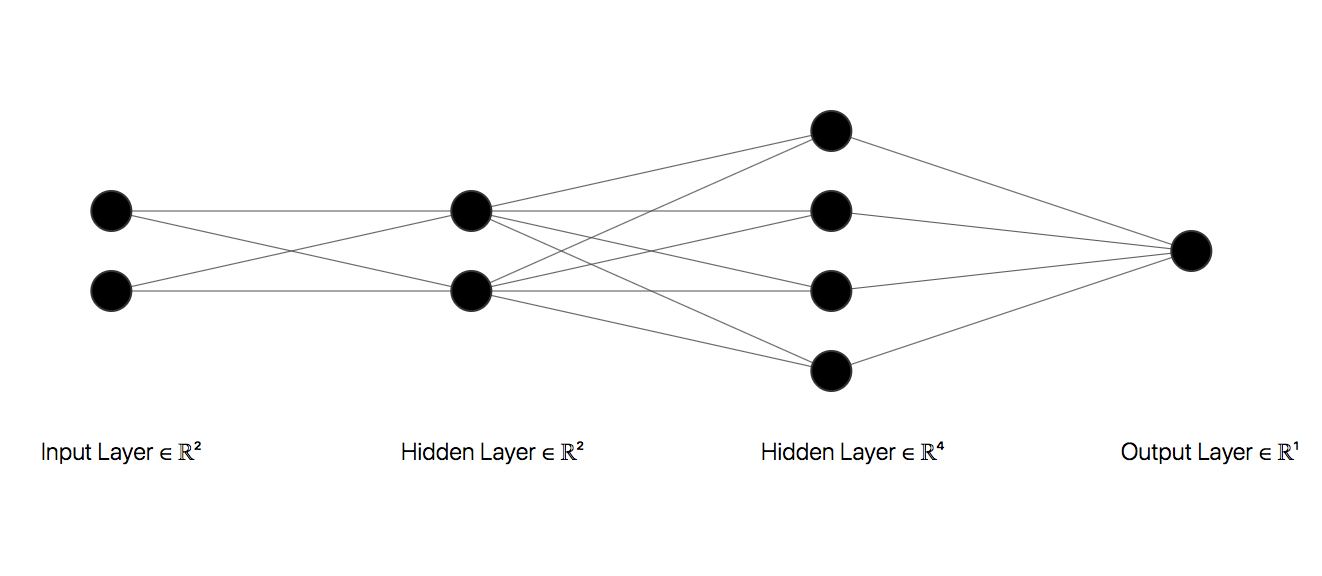
\includegraphics[width=0.5\textwidth]{figures/DNN}
\caption{An example DNN with our architecture with an input dimension of 2}
\label{NN}
 \end{figure}
 \section{Results}
A total of 147 statistically significant ($p < 0.01$) features were found. The total number of features tested was 6480, resulting in 65 features that are expected to be false positives (demonstrating the reason for utilizing PCA). 6480 is derived from 15 channels $\times$ ((5 bands + 1 raw) $\times$ 11 single-channel features $\times$ 6 conditions + (5 bands + 1 raw) $\times$ 1 all-channel feature $\times$ 6 conditions). 
\subsection{Statistical Analysis}
All 12 features showed up at least once as a significant discriminator between our subject groups. Furthermore, every band ($\alpha, \beta, \delta, \gamma, \theta$) and the raw signal produced discriminating features. Table \ref{T1} compares the number of features produced by each condition (the number of expected false positives for each condition is 11) and band combination. Table \ref{T3} breaks down the number of features produced by each channel for each condition. Table \ref{T4} displays feature-channel-band combinations that were significant across at least two conditions. 

While all sub-bands and the raw signal produced significant results, the delta sub-band and the raw signal seemed to be the most effective in discriminating across groups. As an example, figures \ref{delta signal} and \ref{raw signal} demonstrate the difference between the groups’ averaged EEG wave structure and corresponding graph node degree sequence in the Wr channel, all new condition in delta and raw.

\begin{figure}
 \centering
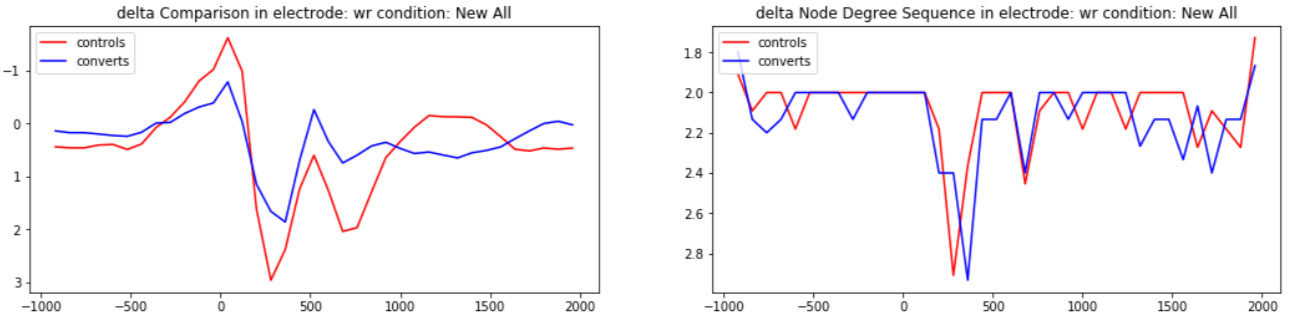
\includegraphics[height=3.5cm,width=8cm]{figures/delta_signal}
\caption{The $\delta$ band averaged time series on the left, corresponding average degree sequences on the right}
\label{delta signal}
 \end{figure}
 
 \begin{figure}
 \centering
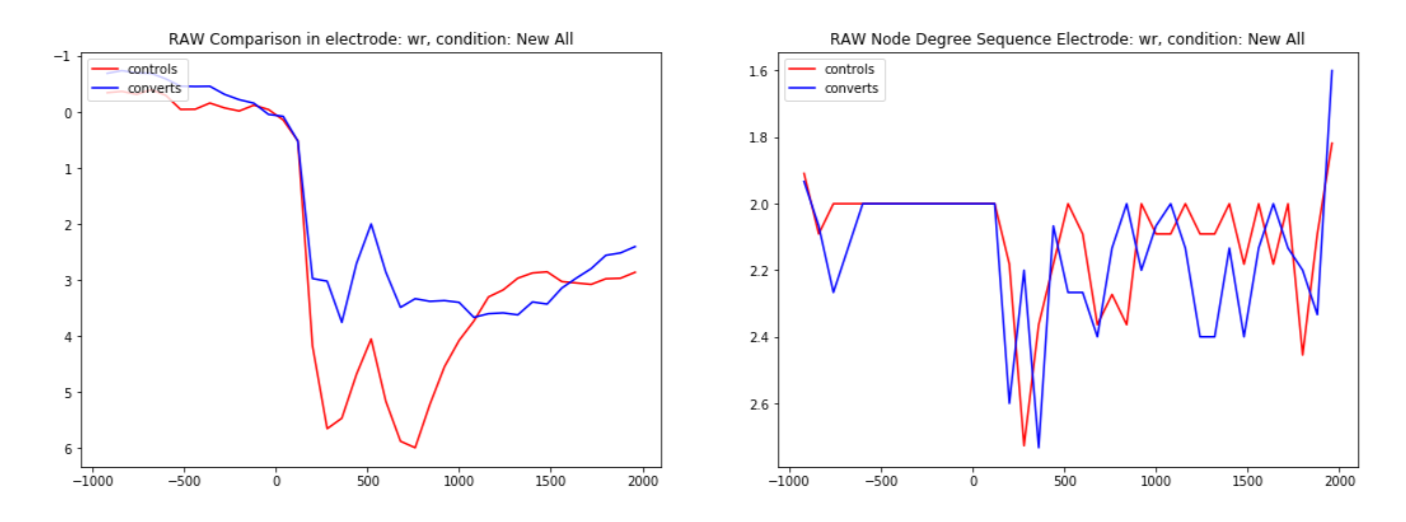
\includegraphics[height=3.7cm,width=8.3cm]{figures/raw_signal}
\caption{The raw band averaged time series on the left, corresponding average degree sequences on the right}
\label{raw signal}
 \end{figure}

\begin{table}
\centering
\footnotesize
\begin{tabular}{l*{7}{c c c c c c | c}r}
Category            & AN & NC & NI & AO & OC  & OI & Total\\
\hline
raw & 1&4&6&8&2&15 & 36\\
$\delta$ & 3 & 5 & 5 & 9 & 4 & 22 & 48\\
$\theta$ &3&6&0&3&2&4 & 18\\
$\alpha$ & 0 & 5 & 1 & 1 & 2 & 2 & 10\\
$\beta$          &  3 & 1 & 5 & 3 & 0 & 1 & 13\\
$\gamma$ & 2&1&0&15&0&3 & 21\\
\hline
total &12&22&17&39&10&47 & 147\\
$E[TP|p<0.01]$ &1&11&6&28&0&36&82\\
\end{tabular}
\caption{Comparing the number of features produced by each band, and the totals. Note: $E[TP| p < 0.01]$ represents the expected number of true positives given our p value}
\label{T1}
\end{table}

\begin{table}
\centering
\begin{tabular}{l*{7}{c}r}
Channel            & AN & NC & NI & AO & OC  & OI &Total\\
\hline
Fz &2&0&0&6&1&2&11\\
Pz &0&1&1&4&2&5&13\\
CZ &0&2&0&5&1&6&14\\
F7 &1&13&0&3&0&0&17\\
F8 &0&1&0&2&0&0&3\\
Bl &0&0&3&0&0&0&3\\
Br &0&0&0&0&0&1&1\\
L41 &1&0&0&2&1&1&5\\
R41 &2&0&3&1&0&4&10\\
Wl &0&0&1&3&2&1&7\\
Wr &3&0&4&3&1&13&24\\
T5 &1&5&0&1&0&3&10\\
T6 &0&0&0&5&0&4&9\\
O1 &1&0&4&3&2&3&13\\
O2 &1&0&0&1&0&4&6\\
CCSS &0&0&1&0&0&0&1
\end{tabular}
\caption{Comparing the number of features produced by each channel for all conditions. Note: CCSS is included as it is not channel specific.}
\label{T3}
\end{table}
\begin{table*}
\centering
\footnotesize
\begin{tabular}{l*{7}{c}r}
Electrode/Conditions (p-value) & AN & NC & NI & AO & OC & OI\\
\hline
Wr: Global Efficiency, Raw, Increase & $7.88 \times 10^{-3}$ & & $4.40 \times 10^-3$ & & $8.31 \times 10^{-3}$ &\\
Wr: GIC, Raw, Increase &&& $2.22 \times 10^-3$ &$9.32 \times 10^-3$& & $6.98 \times 10^-3$ \\
Wr: TSP, Raw, Increase &&&& $6.86 \times 10^-3$ &&$8.20 \times 10^-3$&\\
Wr: Global Efficiency, $\delta$, Increase &&&$8.79 \times 10^-3$&&&$2.13\times10^-4$ \\
R41: GIC, $\delta$, Increase & $8.19\times10^-3$ &&$8.85 \times 10^-3$ &&&$7.91 \times 10^-4$\\
R41: Global Efficiency, $\delta$, Increase &&&$7.71 \times 10^-3$&$2.44\times10^-3$&&$1.78\times10^-3$\\
R41: TSP, $\delta$, Increase &&&$1.97 \times 10^-3$&&&$6.19 \times 10 ^-3$\\
R41: Density, $\delta$, Increase &$3.98 \times 10^-3$&&&&&$1.93 \times 10^-3$\\
O1: Global Efficiency, Raw, Increase &&&$7.63 \times 10^-4$&&$4.23 \times 10^-5$&$1.31 \times 10^-3$\\
O1: Density, Raw, Increase &&&$7.10 \times 10^-3$&&&$6.77 \times 10^-3$ \\
Fz: Global Efficiency, Raw, Increase &$9.70 \times 10^-3$&&&$7.07 \times 10^-4$&&$1.78 \times 10^-3$ \\
Fz: TSP, $\delta$, Increase &&&&$9.03 \times 10^-3$&&$1.75 \times 10^-3$ \\
F7: TSP, Raw, Increase &&$8.83 \times 10^-3$&&&$8.67 \times 10^-3$&\\
Cz: Vertex Coloring, $\delta$, Increase &&$9.64 \times 10^-3$&&&$4.34 \times 10^-4$&\\
Cz: Max Clique, $\gamma$, Decrease &&&&$5.64 \times 10^-3$&&$6.19 \times 10^-3$ \\
T6: Global Efficiency, Raw, Increase &$3.87 \times 10^-3$&&&&&$7.27 \times 10^-3$\\
T6: GIC, Raw, Increase &&&&$4.67 \times 10^-3$&&$2.40 \times 10^-4$ \\
Wl: TSP, $\theta$, Increase &&&&$3.77 \times 10^-4$&&$8.95 \times 10^-3$\\
Pz: Global Efficiency, $\delta$, Increase &&&&&$1.02 \times 10^-3$&$9.25 \times 10^-4$\\
\end{tabular}
\caption{Showing conditions that shared the same significant feature. First column is formatted as Electrode: Feature, Band, Direction of Change. Direction of change is labeled increase if the average value of the feature was higher in the MCI-C group}
\label{T4}
\end{table*}

\begin{table}
\centering
\small
\begin{tabular}{l*{5}{c}r}
Type & Accuracy (\%) & SD (\%) & FP & FN\\
\hline
MCI-C vs RNE & 99.75 & 2.49 & 1 & 0\\
AD & 99.17 & 5.95 & NA & 5
\end{tabular}
\caption{Classification Statistics. FP denotes the number of false positives and FN denotes the number of false negatives}
\label{classification}
\end{table}
\subsection{Classification}
The neural network was trained and evaluated 100 times, each time training on 22 randomly selected participants (85\%) and testing on the remaining 4 participants (15\%). The best results were obtained by reducing the dimension of the feature vector from 147 to 11 via PCA (roughly following the 10\% guideline as suggested in Ahmadlou et al.’s VG EEG analysis \cite{Ahmadlou2010}). As mentioned earlier, the DNN was structured with two hidden layers, the first being the same size as the input layer (11 nodes) and the second being double the first (22 nodes). As 400 classifications were performed, an accuracy of 99.75\% signifies that there were 399 correct classifications and 1 misclassification (1 false positive). This accuracy is significantly higher than similar MCI-C vs RNE classification papers, which result in 71-90\% classification accuracy (\citet{MCI80}, \citet{MCI90}, \citet{MCI71}, \citet{MCI85}). 

Finally, we tested the neural network on a set of 6 diagnosed Alzheimer's patients that were never seen during training to find out whether the features discovered for MCI-C were also applicable to Alzheimer's. The model was trained on the MCI-C patients and then applied to the 6 Alzheimer's patients; this process was run 100 times. The accuracy of classifying AD patients alone (correctness was defined as classifying AD as MCI-C as the model was trained to discriminate between MCI-C and RNE) was 99.17\% with an SD of 5.95\%.

Table \ref{classification} presents the accuracy of classifications.
\section{Verification}
In order to verify the features discovered, we also performed the same feature selection method on the aforementioned set of 6 Alzheimer's patients. Features shared by both groups were then compared to determine which ones can be considered more generalizable. A total of 1820 features were discovered for the Alzheimer's group (28.4\% of tested features). Of the 147 discovered discriminating between MCI-C and RNE, 91 were also present in Alzheimer's testing. Every single channel and band were present in the 91 shared discriminators between MCI-C and Alzheimer's and 11 out of 12 tested features (everything except CCSS) were shared, verifying our results on the MCI-C group.
\section{Discussion and Conclusion}
EEG Analysis of word repetition trials has proven to be an effective method of differentiating between patients with MCI and robust normal elderly (control) patients (\citet{OlichneyN400}, \citet{OlchneyP600}, \citet{TaylorERP}). As a result, we hypothesized that EEG analysis of word repetition trials would produce features that could be utilized for high-accuracy classification between our MCI-C and RNE groups. The recent development of the Visibility Graph allowed for a method of EEG time series graph conversion that encodes many of the characteristics of the original time series. 

Many of the graph features compared across groups were already confirmed to be significant in resting state EEG VG studies, however (unsurprisingly) they were also significant in our analysis of word repetition trials. Novel features introduced in this paper were expected and confirmed via t-testing to encode more differences between our two groups in word repetition trials. But because approximately half of our features could have been produced from type I errors, we only displayed feature-channel combinations that were shared by at least two conditions and we utilized PCA to reduce the number of features used for classification. 

Classification with our DNN structure resulted in a high accuracy of 99.75\% on MCI-C vs Control, and then 99.17\% on an unseen set of 6 Alzheimer's patients. Interestingly, the delta and raw bands seemed to produce the the most amount of features shared by at least two conditions. However our 80 ms epoching could have contributed to these two bands becoming significant and others being less significant. The old incongruous trials condition produced the highest number of results in this comparison. Channels that appeared more than once in this were Wr, R41, O1, Fz, Cz, and T6. This seems to \textbf{CONTRADICT/ALIGN WITH (I DON'T KNOW YET)} our knowledge of group differences in word rep analysis. \textbf{TALK ABOUT THESE CHANNELS HERE AND HOW IT CORRESPONDS TO OTHER RESEARCH}. 
The most common features that appeared in the cross-condition comparison were global efficiency, GIC, TSP cost, and density, and they all were higher in the MCI-C group. These four features can all be interpreted in terms of the complexity of the graph; the number of edges between nodes can create great variation between graphs for these features. This points to a difference in EEG time series structure between groups, especially with regards to voltage differences and overall structure differences in the waveforms, as seen in the examples displayed in figures \ref{delta signal} and \ref{raw signal}.

This paper describes a promising method and set of features for utilizing word rep trials to classify patients who have MCI with great accuracy. While more testing is needed on this method and how it can be used to classify between more groups simultaneously (MCI Non-Converts, for example), the authors hope that word repetition trials could be eventually utilized for automated early diagnosis of dementia diseases in an non-invasive manner with only an EEG machine and a computer.
% \subsection{Mathematics} \textsf{\journalclass} makes the full
% functionality of \AmS\/\TeX\ available. We encourage the use of
% the \verb"align", \verb"gather" and \verb"multline" environments
% for displayed mathematics. \textsf{amsthm} is used for setting
% theorem-like and proof environments. The usual \verb"\newtheorem"
% command needs to be used to set up the environments for your
% particular document.

% \subsection{Figures and tables} \textsf{\journalclass} includes the
% \textsf{graphicx} package for handling figures.

% Figures are called in as follows:
% \begin{verbatim}
% \begin{figure}
% \centering
% \includegraphics{<figure name>}
% \caption{<Figure caption>}
% \end{figure}
% \end{verbatim}

% For further details on how to size figures, etc., with the
% \textsf{graphicx} package see, for example, \cite{R1}
% or \cite{R3}.

% The standard coding for a table is shown in Figure~\ref{F2}.

% \begin{figure}
% \setlength{\fboxsep}{0pt}%
% \setlength{\fboxrule}{0pt}%
% \begin{center}
% \begin{boxedverbatim}
% \begin{table}
% \small\sf\centering
% \caption{<Table caption.>}
% \begin{tabular}{<table alignment>}
% \toprule
% <column headings>\\
% \midrule
% <table entries
% (separated by & as usual)>\\
% <table entries>\\
% .
% .
% .\\
% \bottomrule
% \end{tabular}
% \end{table}
% \end{boxedverbatim}
% \end{center}
% \caption{Example table layout.\label{F2}}
% \end{figure}

% \subsection{Cross-referencing}
% The use of the \LaTeX\ cross-reference system
% for figures, tables, equations, etc., is encouraged
% (using \verb"\ref{<name>}" and \verb"\label{<name>}").

% \subsection{End of paper special sections}
% Depending on the requirements of the journal that you are submitting to,
% there are macros defined to typeset various special sections.

% The commands available are:
% \begin{verbatim}
% \begin{acks}
% To typeset an
%   "Acknowledgements" section.
% \end{acks}
% \end{verbatim}

% \begin{verbatim}
% \begin{biog}
% To typeset an
%   "Author biography" section.
% \end{biog}
% \end{verbatim}

% \begin{verbatim}
% \begin{biogs}
% To typeset an
%   "Author Biographies" section.
% \end{biogs}
% \end{verbatim}

% %\newpage

% \begin{verbatim}
% \begin{dci}
% To typeset a "Declaration of
%   conflicting interests" section.
% \end{dci}
% \end{verbatim}

% \begin{verbatim}
% \begin{funding}
% To typeset a "Funding" section.
% \end{funding}
% \end{verbatim}

% \begin{verbatim}
% \begin{sm}
% To typeset a
%   "Supplemental material" section.
% \end{sm}
% \end{verbatim}


% \subsection{References}
% Please note that the files \textsf{SageH.bst} and \textsf{SageV.bst} are included with the class file
% for those authors using \BibTeX.
% The files work in a completely standard way, and you just need to uncomment one of the lines in the below example depending on what style you require:
%%Harvard (name/date)
\bibliography{bibliography}
\bibliographystyle{SageH}
%%Vancouver (numbered)
%\bibliographystyle{SageV}
%and remember to add the relevant option to the 
% \verb+\documentclass[]{sagej}+ line as listed in Table. 

%\section{Support for \textsf{\journalclass}}
%We offer on-line support to participating authors. Please contact
%us via e-mail at \dots
%
%We would welcome any feedback, positive or otherwise, on your
%experiences of using \textsf{\journalclass}
\subsection{Copyright}
Copyright \copyright\ \volumeyear\ SAGE Publications Ltd,
1 Oliver's Yard, 55 City Road, London, EC1Y~1SP, UK. All
rights reserved.

\begin{acks}

\end{acks}

\end{document}
